\chapter{Formáty využívající se v API}
V této kapitole budou popsány především dva základní formáty dat které jsou stále aktivní. A to JSON a XML.

\section{JSON}
JavaSctript Object Notation neboli JSON je formát který je odvozen z Javascriptu. Nicméně mnoho dnešních jazyků už má zabudovanou serializaci do JSONU. Jedná se o textový formát zápisu objektů který je dobře čitelný člověkem. Bohužel nemá podporu komentářů oproti XML které tuto podporu má. Ukládá data do párů \textbf{key:value} kdy value může být i další objekt nebo pole. Znaky v JSONu musí být v kódování UTF-8 ale podporuje i speciální znaky pokud jsou tzv. escaped. Například \verb |\uD83D\uDE10| \textit{neutral-face} . Je využíván primárně k výměně dat mezi webovými aplikacemi a  servery. Má jednoduchá ale zato striktní pravidla a tudíž je jednoduché zkontrolovat jeho správnost. \textbf{odkaz někde na iso normu https://www.iso.org/standard/71616.html} %TODO bibtech na iso normu plus dát emoji 😐 třeba xetex ale to se pak celé rozbije


\subsection{Pravidla}
\textbf{Key} je vždycky string a reprezentuje atribut. \textbf{Value} je hodnota kterou nabývá key a může být text, číslo, logická hodnota, null, další objekt či pole. Jednotlivé atributy jsou vždy odděleny čárkou. Jako příklad máme JSON objekt z našeho API. Tento objekt popisuje hráče, jeho vlastnosti a navíc jeho rasu.

\newpage

\begin{listing}
  \inputminted{json}{resources/code/player.json}
  \caption{Příklad JSON souboru}
  \label{code:json_player}
\end{listing}

V tomto JSONu máme všechno s čím se můžeme potkat. Jako první máme \verb|"ID":4|. ID je klíč a 4 je číslo. To značí že tento objekt má svůj unikátní identifikátor 4. Může se ovšem stát že by naše číslo 4 bylo v uvozovkách \verb|"4"|. To by pak bylo ohodnoceno jako text ne jako číslo a kdybychom s tím dále chtěli pracovat jako s číslem tak si ho musíme v programu přetypovat. \textbf{idk jestli to tu tento příklad dávat } S tím se také pojí deserializace když chceme převádět JSON zpátky na objekt tak datové typy v objektu musí sedět s těmi co jsou v JSONu.

Dále zde máme na 6 řádku \verb|"title":"Elf"|. Value je v tomto případě text. Taktéž tento řádek v kontextu objektu nám značí že je to rasa která má název Elf.

O dva řádky výše je \verb|"race":{<vlastnosti>}|. To je příklad objektu. v tomto případě rasy a ta má nějaké své vlastnosti.

V key \texttt{"effects"} se nachází pole objektů. V tomto případě to jsou klíče co určují rasu a její efekt plus od jaké úrovně je tento efekt zpřístupněn. Stejně tak na řádku 26 je jako value pole textových řetězců. V tomto případě se jedná o inventář hráče a jeho předměty.

A v neposlední řadě máme na řádku 3 jako value \texttt{null}. To nám značí že tento konkrétní key u tohoto objektu zatím nic neobsahuje. Může se stát že v budoucnu nějakou value dostane nebo může existovat u jiného objektu.

A nakonec zde máme na řádku 29 jako value \texttt{false}. To značí logickou hodnotu a tato value má datový typ boolean. V našem případě se jedná o vlastnost která nám říká zda je hráč mrtvý (\texttt{false}) či nikoli (\texttt{true}).


\section{XML}
Extensible Markup Language je jazyk primárně určený na serializaci a přenášení dat. Stejně jako JSON je čitelný i člověkem. Základní stavební blok je node. Atributy pak ukládá do párů kterým říkáme tagy. Za pomocí své deklarace podporuje určení kódování a různé verze. Také za pomocí XML Schema definition podporuje celou řadu datových typů. Oproti JSONu je zde podpora komentářů. Standardy spravuje W3C \textbf{fest fajny odkaz na w3c specifikaci do bibtex} %TODO bibtech na w3c


\subsection{Pravidla}
Na začátku dokumentu je vždycky XML deklarace, která určuje o jakou verzi se jedná a jaké mají znaky kódování.
Tag je párová značka. Zapisuje se jako počáteční tag (<character>) a ukončovací (</character>) kde \textit{character} je název atributu podobě jako u JSONu \textbf{key}. Hodnota atributu se píše právě mezi počáteční a ukončovací tag. Taktéž se může psát přímo do tagu <character id=4>. Tomuto páru tagů říkáme \textbf{element}. Tzv. \textit{procesory} analyzují XML dokumenty a posílají dále strukturovaná data aplikaci. Procesory můžou být jak validující tak nevalidující. Pokud jde o validující procesor, musí chybu nahlásit ale pořád může pokračovat.


\begin{listing}
  \inputminted{xml}{resources/code/player.xml}
  \caption{Příklad XML dokumentu i se schématem}
  \label{code:xml_player}
\end{listing}

%TODO nějaký odkaz pěkný nebo tak něco na 
Tento XML dokument reprezentuje stejnou strukturu jako JSON zmíněný výše. Je zde navíc na první pohled schéma ve kterém můžeme určit jeden z mnoha \ref{fig:xml_datatypes} datových typů pro každý element (řádek 3) či atribut (řádek 6 a 7). Když není specifikováno schéma tak všechny datové typy jsou pouze text. Taky velká změna oproti JSONu je že víme o jaký objekt se jedná (řádek 23 a 48). Místo obyčejných složených závorek zde máme element který se jmenuje character. Předtím jsme tuto informaci v JSONu nedostali.

\begin{figure}[H]
  \centering
  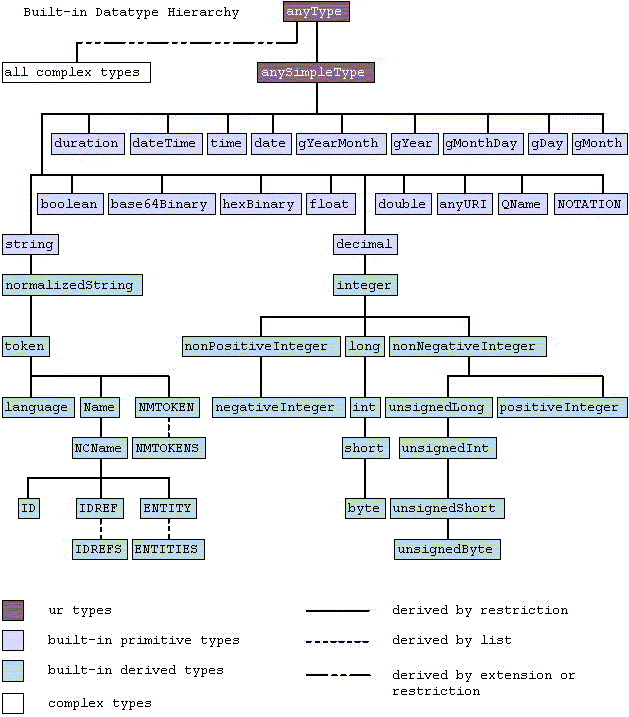
\includegraphics[width=0.7\textwidth]{figures/type-hierarchy.png}
  \caption{Hierarchie datových typů v XML schema}%\cite{british_museum_2021}}
  \label{fig:xml_datatypes}
\end{figure}
%TODO odkaz na obrázek všech možných datových typů https://www.w3.org/TR/xmlschema-2/type-hierarchy.gif a přímo ta stránka https://www.w3.org/TR/xmlschema-2/#built-in-datatypes


\endinput